\documentclass[runningheads,a4paper]{llncs}

\usepackage{amssymb}
\setcounter{tocdepth}{3}
\usepackage{graphicx}
\usepackage{subcaption}
\captionsetup{compatibility=false}

\usepackage{url}   
\newcommand{\keywords}[1]{\par\addvspace\baselineskip
\noindent\keywordname\enspace\ignorespaces#1}

\begin{document}

\mainmatter  % start of an individual contribution

% first the title is needed
\title{Speed estimation for vehicles using \\SVM classification and edge detection}

% a short form should be given in case it is too long for the running head
\titlerunning{Speed estimation for vehicles using SVM classification and edge detection}

% the name(s) of the author(s) follow(s) next
%
% NB: Chinese authors should write their first names(s) in front of
% their surnames. This ensures that the names appear correctly in
% the running heads and the author index.
%
\author{Mathias Dierickx\and Tim Ranson\and Maarten Tindemans\and Bjorn Vandenbussche}
%
\authorrunning{Speed estimation for vehicles using SVM classification and edge detection}
% (feature abused for this document to repeat the title also on left hand pages)

% the affiliations are given next; don't give your e-mail address
% unless you accept that it will be published
\institute{Ghent University, Faculty of Engineering and Architecture\\
Valentin Vaerwyckweg 1, 9000, Ghent}

%
% NB: a more complex sample for affiliations and the mapping to the
% corresponding authors can be found in the file "llncs.dem"
% (search for the string "\mainmatter" where a contribution starts).
% "llncs.dem" accompanies the document class "llncs.cls".
%

\maketitle


\begin{abstract}
This is the abstract: TODO
\keywords{SVM classification, Local Binary Patterns, line detection}
\end{abstract}


\section{Introduction}
TODO

\section{Background}
\subsection{Texture analysis using Local Binary Patterns}
Local Binary Patterns (LBP) \cite{Huang2011} is a non-parametric descriptor whose aim is to efficiently summarize the local structures of images. As a non-parametric method, LBP summarizes local structures of images efficiently by comparing each pixel with its neighboring pixels. The most important properties of LBP are its tolerance regarding monotonic illumination changes and its computational simplicity. LBP was originally proposed for texture analysis \cite{Ojala1996}, and has proved a simple yet powerful approach to describe local structures. 

The original LBP operator labels the pixels of an image with
decimal numbers, called Local Binary Patterns or LBP codes, which encode the local structure around each pixel (see figure \ref{fig:lbp}). Each pixel is then compared with its eight neighbors in a 3x3 neighborhood by subtracting the center pixel value. The resulting strictly negative values are encoded with 0 and the others with 1. A binary number is obtained by concatenating all these binary codes in a clockwise direction starting from the top-left one and its corresponding decimal value is used for labeling. The derived binary numbers are referred to as Local Binary Patterns or LBP codes. 

One limitation of the basic LBP operator is that its small 3x3 neighborhood cannot capture dominant features with large scale structures. To deal with the texture at different scales, the operator was later generalized to use neighborhoods of different sizes \cite{Ojala}. The histogram of LBP labels can then be exploited as a texture descriptor.

\begin{figure}[h]
\centering
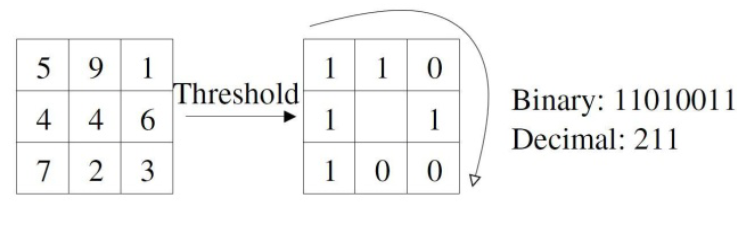
\includegraphics[height=3cm]{fig/LBP.png}
\caption{An example of the basic LBP operator}
\label{fig:lbp}
\end{figure}

\subsection{SVM classification}
Support Vector Machines (SVM's) \cite{Boswell2002} are a learning method used for binary classification. The idea is to find a hyperplane which separates the $d$-dimensional data perfectly into its two classes. However, since example data is often not linearly separable, SVM's introduce the notion of a "kernel induced feature space" which casts the data into a higher dimensional space where the data is separable. Typically, casting into such a space would cause problems computationally, and with overfitting. The key insight used in SVM's is that the higher-dimensional space doesn't need to be dealt with directly, which eliminates the above concerns.

Basically, we want the hyperplane that maximizes the geometric distance to the closest data points (as shown in figure \ref{fig:hyperplane}).

\begin{figure}[h]
\centering
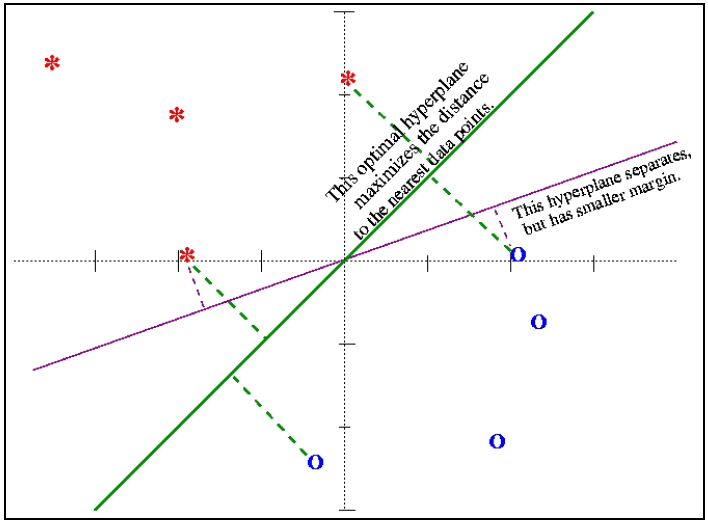
\includegraphics[height=7cm]{fig/SVM_hyperplane.png}
\caption{Choosing the hyperplane that maximizes the margin.}
\label{fig:hyperplane}
\end{figure}

Only the closest data points contribute to deciding the optimal hyperplane, which is why these are called the \textit{support vectors}. They are the only ones needed in defining (and finding) the optimal hyperplane. 

The equation for the hyperplane is subject to a constraint concerning the parameter $C$. 
One can think of $C$ as a tunable parameter: higher $C$ corresponds to more importance on classifying all the training data correctly, lower $C$ results in a more "flexible" hyperplane that tries to minimize the margin error for each example.

\paragraph{Kernels} The original equation for the hyperplane to linearly separate the data contains a linear kernel. \cite{Hsu2016} points out when the use of a simple linear kernel is appropriate:
if the number of features is large, one may not need to map data to a higher dimensional space. That is, the nonlinear mapping does not improve the performance. Using the linear kernel is good enough, and one only searches for the parameter $C$.

We mentioned that SVM's can use a "kernel induced feature space" which casts the data into a higher dimensional space where the data is separable, in case the data is not linearly separable in its original space. Pending on the type of data and application of the SVM, there are several types of kernels which could be used. The Radial Basis Function (RBF) kernel is a often a reasonable first choice, because it can handle the case when the relation between class labels and attributes is non-linear, while only adding one more parameter $\gamma$ to search for.

\paragraph{Parameters} There are two parameters for an RBF kernel: $C$ and $\gamma$. It is not known beforehand which $C$ and $\gamma$ are best for a given problem; consequently some kind of model selection (parameter search) must be done. The goal is to identify good ($C$, $\gamma$) so that the classifier can accurately predict unknown data (i.e. testing data).

One method for comparing results for a set of parameter values is cross-validation. In $v$-fold cross-validation, we first divide the training set into $v$ subsets of equal size. Sequentially one subset is tested using the classifier trained on the remaining $v − 1$ subsets. Thus, each instance of the whole training set is predicted once so the cross-validation accuracy is the percentage of data which are correctly classified.

\subsection{Precision, recall, F-scores}

TODO: Bjorn

\subsection{Line detection}
TODO: Mathias


\section{Method}
In order to determine the maximum speed of a vehicle two image processing techniques are used: SVM classification and edge detection. We first try to rely on edge detection to find the contours of the lanes where driving is permitted (i.e. where no obstacles are found). We estimate the reliability of the edge detection and incorporate road detection using the SVM classifier when needed.

For the implementation of our method, we use OpenCV 3.1 \cite{Bradski2000} and C++. Four different datasets were used to either train or test the solution.
To train out SVM classifier, we used a function of the OpenCV SVM library which selects the optimal parameters using cross-validation.

\subsection{Parameters for SVM classification}\label{parameters-classification}
The goal of this classifier is to determine what pixels are part of the road and which are not. We will describe multiple tunable parameters in order to get optimal classification for road detection. These parameters determine both the length and values of the feature vectors, which are then fed to the SVM classifier. We compare classification results varying these parameters for the feature vector in section \ref{results-svm-classification}.

\subsubsection{Block size}
Each frame is split into multiple blocks of predetermined size. We chose to vary the block sizes between 8x8px, 16x16px and 32x32px. On the one hand, larger block sizes would too easily contain multiple structures of different classes, resulting in poorer classification. For example a block on the edge of the road containing part of the street and grass. On the other hand, smaller block sizes would omit too many details to be descriptive enough to use for classification.

The block size affects the level of detail taken into account while calculating the feature vector, as the values for the feature vector operate within one block size. Some examples of different block sizes can be found in figure \ref{fig:methods-block-sizes}.

\begin{figure}[ht]
\centering
\begin{subfigure}{.49\textwidth}
  \centering
  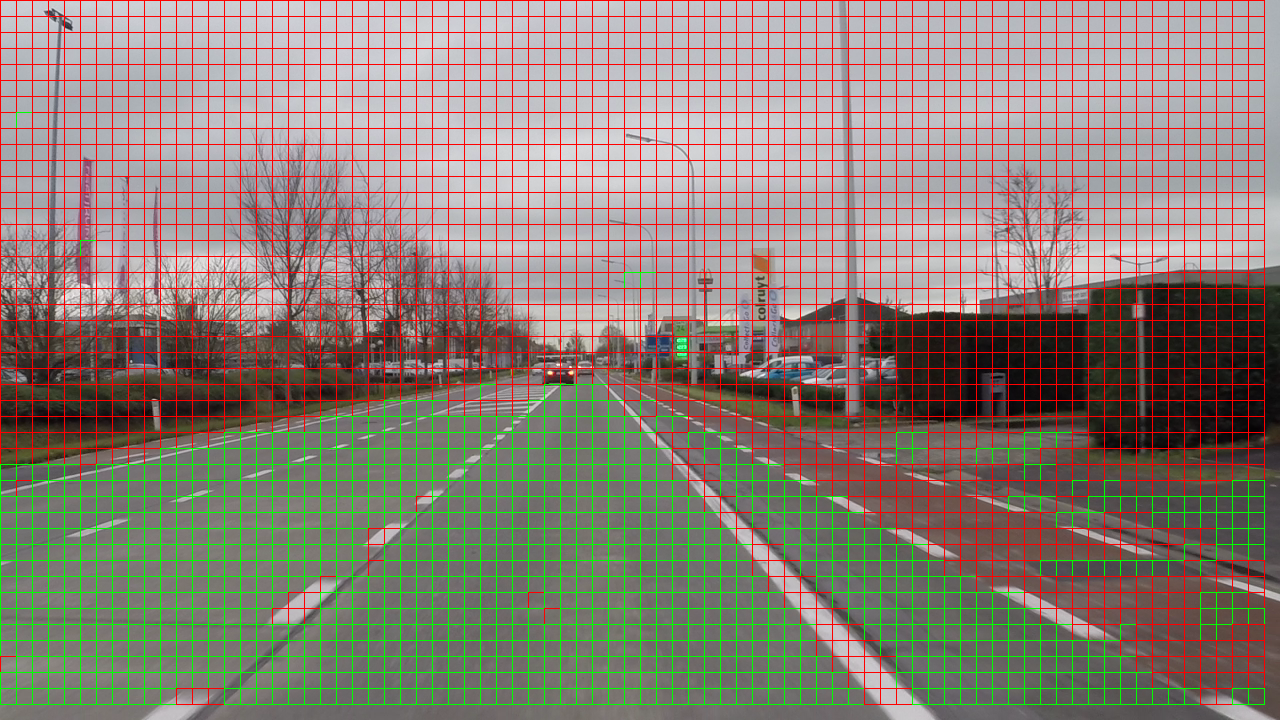
\includegraphics[width=1\textwidth]{fig/svm_prediction_16_lbp_marks.png}
  \caption{Block size 16x16px}
\end{subfigure}
\begin{subfigure}{.49\textwidth}
  \centering
  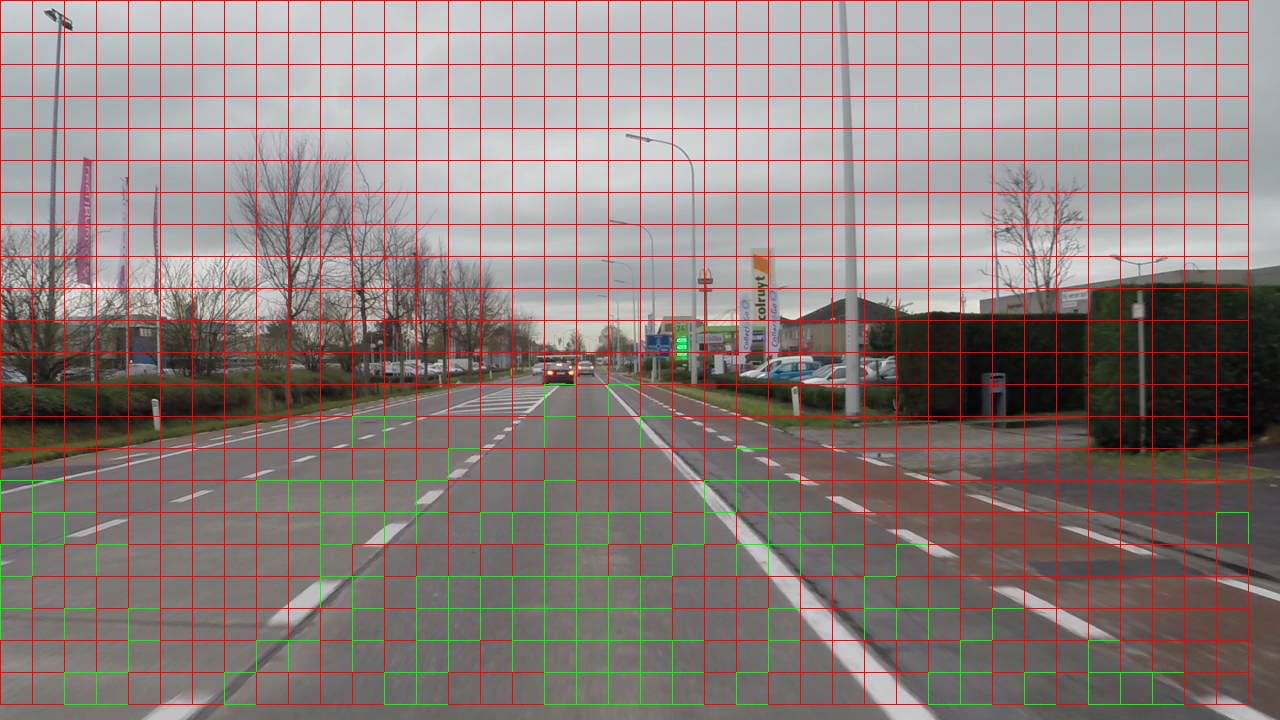
\includegraphics[width=1\textwidth]{fig/svm_prediction_32_lbp_marks.png}
  \caption{Block size 32x32px}
\end{subfigure}
\caption{SVM prediction using only LBP values and including road marks. Green blocks were predicted to be road, red to be non-road.}
\label{fig:methods-block-sizes}
\end{figure}

\subsubsection{LBP}
With LBP we try to characterize the structure of roads within a block. The histogram of LBP values within that block can be added to the feature vector in order to improve classification. These histograms are calculated per channel (e.g. 3 channels for RGB) and are added consecutively to the feature vector. 


\subsubsection{Color}
Because working with LBP values only doesn't take color intensity into account \cite{Pietikainen2002}, histogram values of color intensity per block and channel are added to the feature vector. 

\subsection{Kernels for SVM classification}\label{methods-kernels}
Judging from the OpenCV documentation\footnote{http://docs.opencv.org/3.1.0/} there are two SVM kernels fit for a two-class classification problem.
A linear kernel is faster, but the RBF kernel will outperform the linear kernel in case the data is not linearly separable. We tested and compared the results using each kernel to decide which is best fit for our classification problem.

\subsection{Training the SVM classifier}
For each combination of the previously mentioned parameters, the SVM classifier must be trained. For a training set (a subset of the datasets available) each frame is divided into blocks. Each block must be manually labelled with the expected value for classification. For practical reasons we put a margin between each block in the frames of the training set and only used the $i$-th frame of each dataset (i=0,10,...,40).
Figure \ref{fig:frame-training} shows a visualization of pre-labeled blocks in a frame.
The classifier is trained using the label and calculated feature vector for each block in each frame of the training set.

\begin{figure}[ht]
\centering
  \centering
  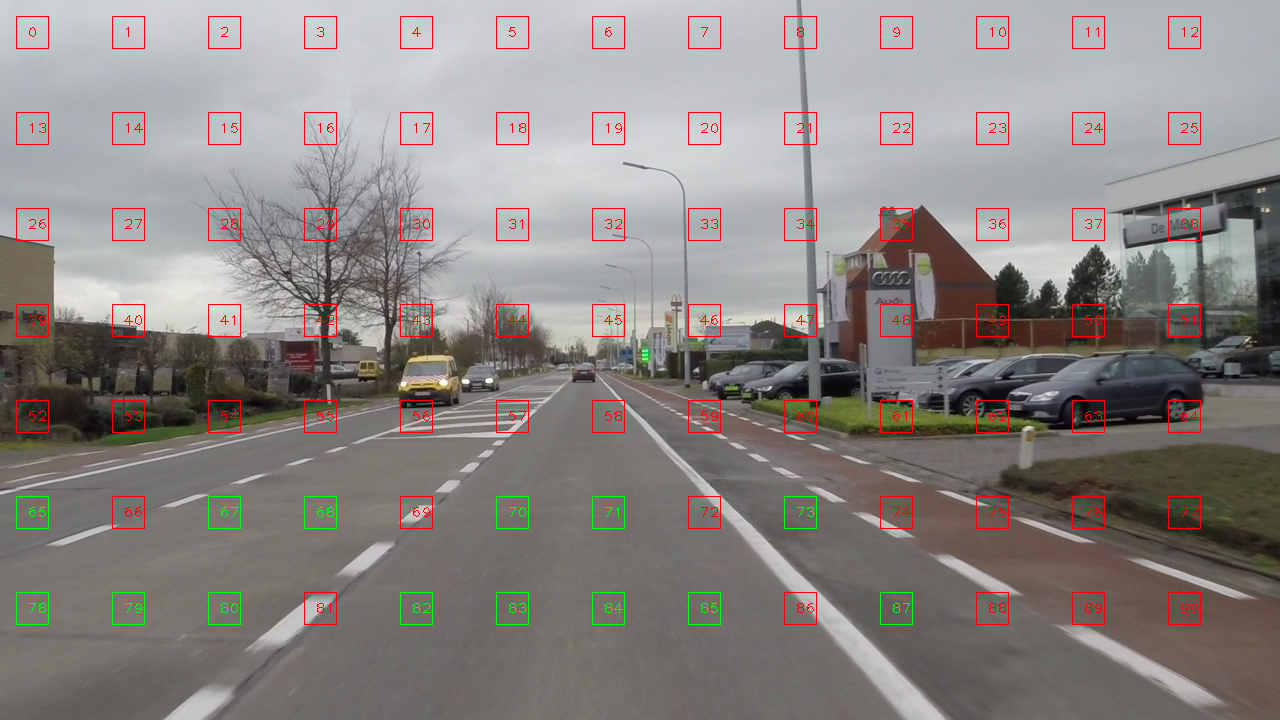
\includegraphics[width=.7\textwidth]{fig/svm_training_32.png}
\caption{Visualization of a pre-labelled frame of a training set. Block size 32x32px, excluding road marks}
\label{fig:frame-training}
\end{figure}

\subsection{Road marks}
The training dataset was labelled considering blocks containing road marks once as part of the road class and once as part of the non-road class. Initially road marks were labelled as non-road, in order to get a good classification of road (i.e. different types of asphalt). As these road marks aren't really considered an obstacle for a car driver, ideally they should be classified as road. This makes up for a more difficult classification problem. To quantify this effect we apply classification both with and without road marks. 

\subsection{Removing details}

Detecting edges is very straightforward using an edge detection algorithm like Canny Edge Detection \cite{canny}. However, there are a lot of edges on the road itself, thinking of road markings and cobbles. The edges on the road, considered as noise, and the edges of the road are not unambiguously separable. The width of the patterns that cause the edges on the road is rather small. Using morphological image processing operations, it is possible to remove these small patterns.  In figure \ref{cobbles_erode_out}, a smoothed cobbled road is shown.
\begin{figure}[ht]
\centering
\begin{subfigure}{.5\textwidth}
  \centering
  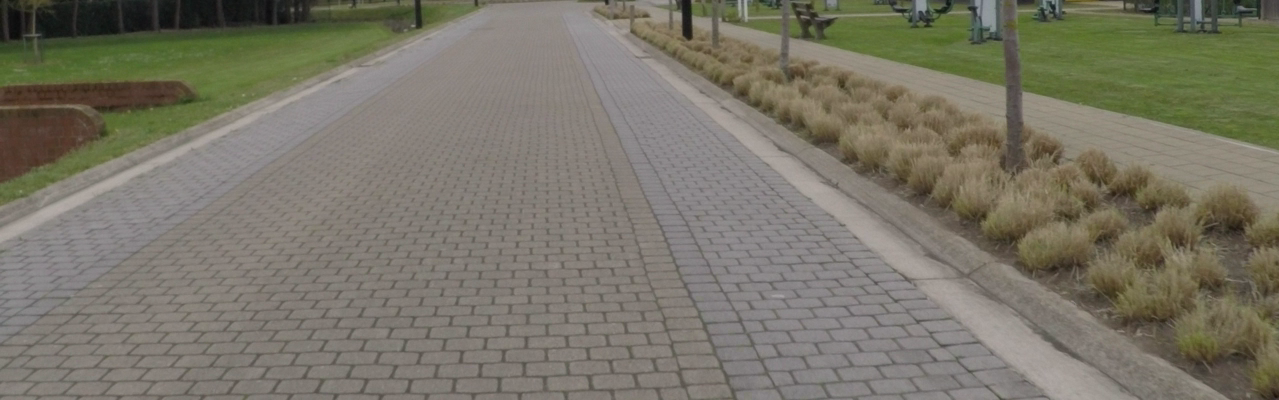
\includegraphics[width=.9\textwidth]{fig/cobbles_in.png}
  \caption{Original frame\label{cobbles_in}}
\end{subfigure}%
\begin{subfigure}{.5\textwidth}
  \centering
  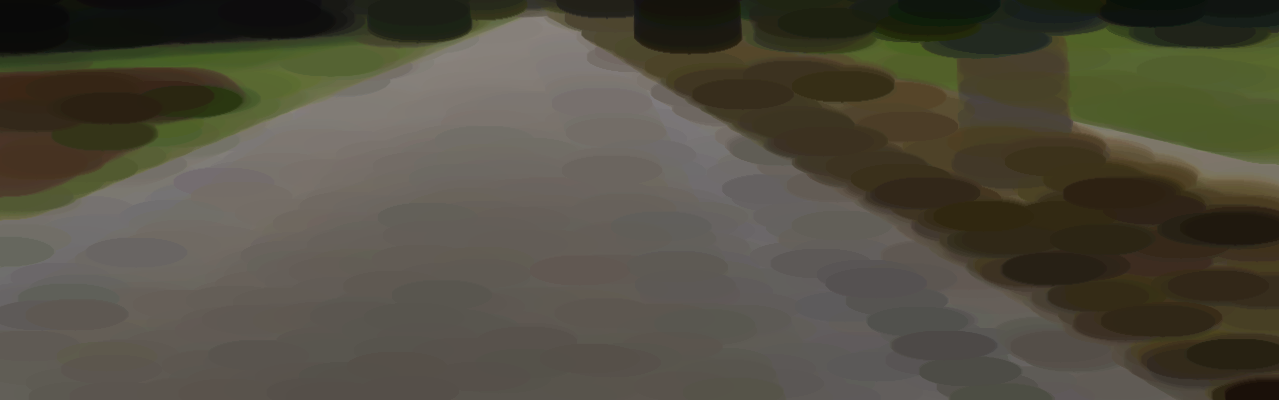
\includegraphics[width=.9\textwidth]{fig/cobbles_erode_out.png}
  \caption{Eroded cobbled road\label{cobbles_erode_out}}
\end{subfigure}
\caption{Perform eroding to remove the edges on the road.}
\end{figure}

Eroding is a morphology operator to make the objects on the foreground, which are the brightest, smaller \cite{sreedhar2012enhancement}. Figure \ref{line_zoom_eroded} shows an example of a thinned white line. When the kernel is large enough, white lines can be filtered out completely. The same technique is used to smooth the surface of cobbled roads. A cobblestone consist of a bright center, surrounded by darker joints. By eroding the cobbled road, the erode function will minimize the center of the cobble, which will cause enlarged joints. With a large kernel, the joints will spread until they overlap. The best results were achieved with an ellipsoidal kernel of 100 x 30 px.

\begin{figure}[ht]
	\begin{minipage}[t]{.45\textwidth}
		\centering
		\begin{subfigure}[t]{.5\textwidth}
		  \centering
		  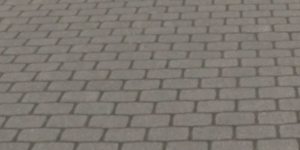
\includegraphics[width=.9\textwidth]{fig/cobbles_zoom_original.png}
		  \caption{Original frame\label{cobbles_zoom_original}}
		\end{subfigure}%
		\begin{subfigure}[t]{.5\textwidth}
		  \centering
		  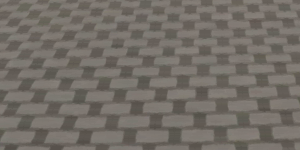
\includegraphics[width=.9\textwidth]{fig/cobbles_zoom_eroded.png}
		  \caption{Bigger joints after eroding\label{cobbles_zoom_eroded}}
		\end{subfigure}
		\caption{The effect of eroding cobbled roads.}
	\end{minipage}%
	\hspace{0.05\textwidth}
	\begin{minipage}[t]{.45\textwidth}
		\centering
		\begin{subfigure}[t]{.5\textwidth}
		  \centering
		  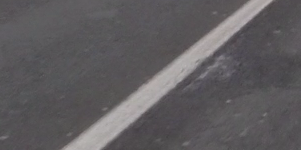
\includegraphics[width=.9\textwidth]{fig/line_zoom_original.png}
		  \caption{Original frame\label{line_zoom_original}}
		\end{subfigure}%
		\begin{subfigure}[t]{.5\textwidth}
		  \centering
		  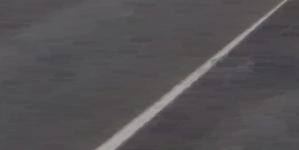
\includegraphics[width=.9\textwidth]{fig/line_zoom_eroded.png}
		  \caption{Smaller lines after eroding\label{line_zoom_eroded}}
		\end{subfigure}
		\caption{The effect of eroding road markings.}
	\end{minipage}
\end{figure}

Unfortunately, the erode function will cause the darker objects to expand. The original size of the objects has been modified, as seen in \ref{car_erode_bigger}. This will falsify the eventual edge detection. In this example, the observed car is reported to close. In order to restore the original measures, dilation is executed. This is the opposite morphology operator of eroding. The combination of eroding and dilation is called opening. When dilation is executed with the same kernel size of the erode function, the original size of the dark objects will decrease to their original size, as seen in \ref{car_dilate_smaller}. Note that, after eroding, some details of the shape of the objects are lost. In order to provide a safety margin, the dilate function is executed with a slightly smaller kernel.


\begin{figure}[ht]
\centering
\begin{subfigure}{.5\textwidth}
  \centering
  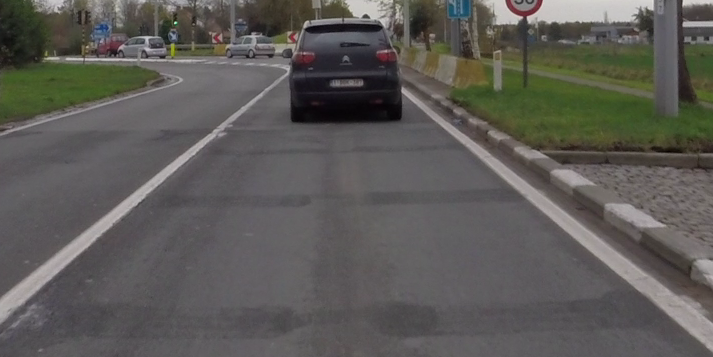
\includegraphics[width=.9\textwidth]{fig/car_original.png}
  \caption{Original frame\label{car_original}}
\end{subfigure}%
\begin{subfigure}{.5\textwidth}
  \centering
  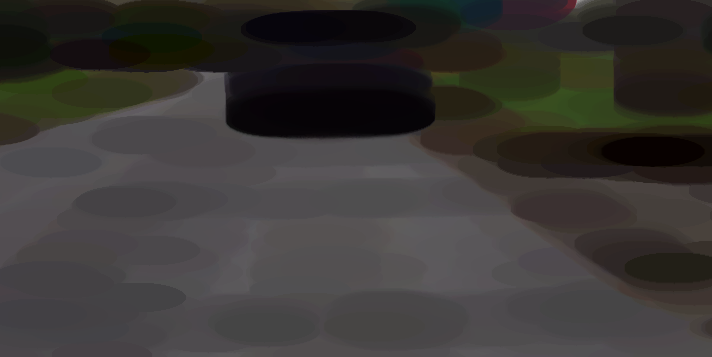
\includegraphics[width=.9\textwidth]{fig/car_erode_bigger.png}
  \caption{Dark objects are bigger after eroding\label{car_erode_bigger}}
\end{subfigure}
\begin{subfigure}{.5\textwidth}
  \centering
  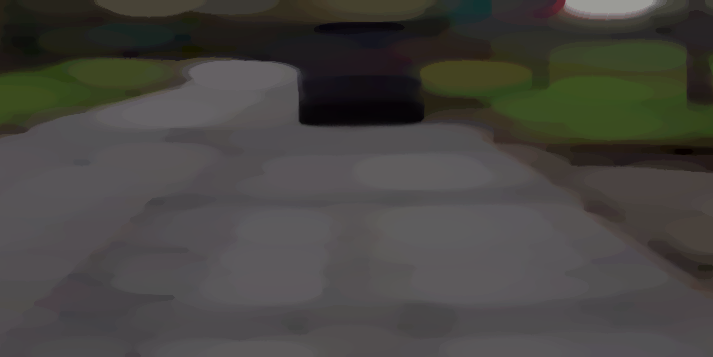
\includegraphics[width=.9\textwidth]{fig/car_dilate_smaller.png}
  \caption{Restore original sizes with dilation\label{car_dilate_smaller}}
\end{subfigure}
\caption{Perform eroding and dilation to remove details.}
\end{figure}

\subsection{Canny Edge Detection}

To detect the edges of the road, the Canny Edge Detection algorithm is used. Figure \ref{canny_edges} shows an example. 


\begin{figure}[ht]
	\centering
	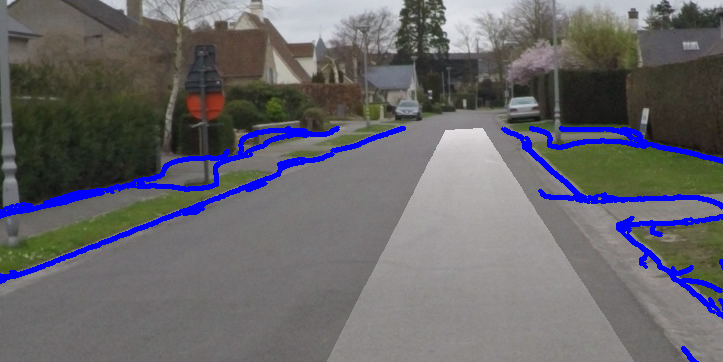
\includegraphics[width=.5\textwidth]{fig/canny_edges.png}
	\caption{Canny edge detection\label{canny_edges}}
\end{figure}

This algorithm requires a minimum and a maximum threshold value, which were determined experimentally. 
The best results were achieved with a maximum threshold that is twice the minimum threshold.
The minimum threshold is determined by the required minimum sensitivity. When the algorithm is configured too sensitive, some imperfections on the road will be detected as edges. On the other hand, a certain level of sensitivity is necessary to detect less clear road edges. For example, a transition from road to dirt has a very small distinction of color and brightness, as seen in \ref{transition_road_dirt_eroded}. The minimum threshold should be high enough to detect this transition as edge. 

\begin{figure}[ht]
\centering
\begin{subfigure}{.5\textwidth}
  \centering
  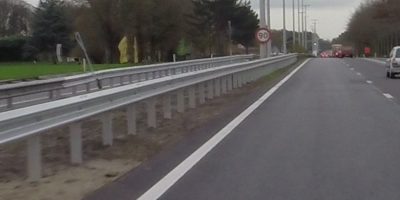
\includegraphics[width=.9\textwidth]{fig/transition_road_dirt_original.png}
  \caption{Original frame\label{transition_road_dirt_original}}
\end{subfigure}%
\begin{subfigure}{.5\textwidth}
  \centering
  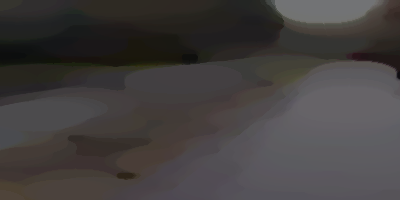
\includegraphics[width=.9\textwidth]{fig/transition_road_dirt_eroded.png}
  \caption{Eroded road\label{transition_road_dirt_eroded}}
\end{subfigure}
\caption{Unclear transition from road to non-road.}
\end{figure}

\subsection{Zebra crossings}
TODO

\subsection{Combination of classification and edge detection}\label{method-combination}

For each frame the given masks show the projected trajectory of the car. Intersections get calculated in order to find the road where it's safe to drive. The edges of the edge detection are visualized as blue lines on figure \ref{visualization}. The intersections are shown in green. The closest intersection to the car is shown in red. At this point the maximum speed is derived from the intensity of this pixel. 

In order to calculate the edges, both road classification and edge detection are combined. Therefor two strategies were tested:
\begin{enumerate}
\item  A region is considered to be road only if it's identified as road by the road classification and there are no edges. Both classification and edge detection should indicate a pixel as road in order to be used for safe driving.
\item A region is considered to be road if there are no edges. When edges are detected, road classification is used to decide what part of the image is road. 
\end{enumerate} 

Both strategies start by removing outliers from the road classification. The goal of this is to eliminate the effect an outlier would have when it's close to the car. A non-road block is considered an outlier when it has less than 4 non-road block neighbours. This is repeated until all outliers are removed.

For the first strategy the edges of the classification are computed. These get combined with the edges from the edge detection. The closest intersection of any edge with the given mask of the image is used to calculate the maximum speed of the vehicle.

In the second strategy, the edges are checked if they aren't on the road. This is done by checking that an edge is on a non-road block of the road classification. For safety reasons there is an additional check. The above, left and right blocks of an edge should also be considered as non-road. When the edge is not classified as road, it is added to a collection. The intersections of the edges in the collection and the masks are then computed. 

\begin{figure}[t]
  \centering
  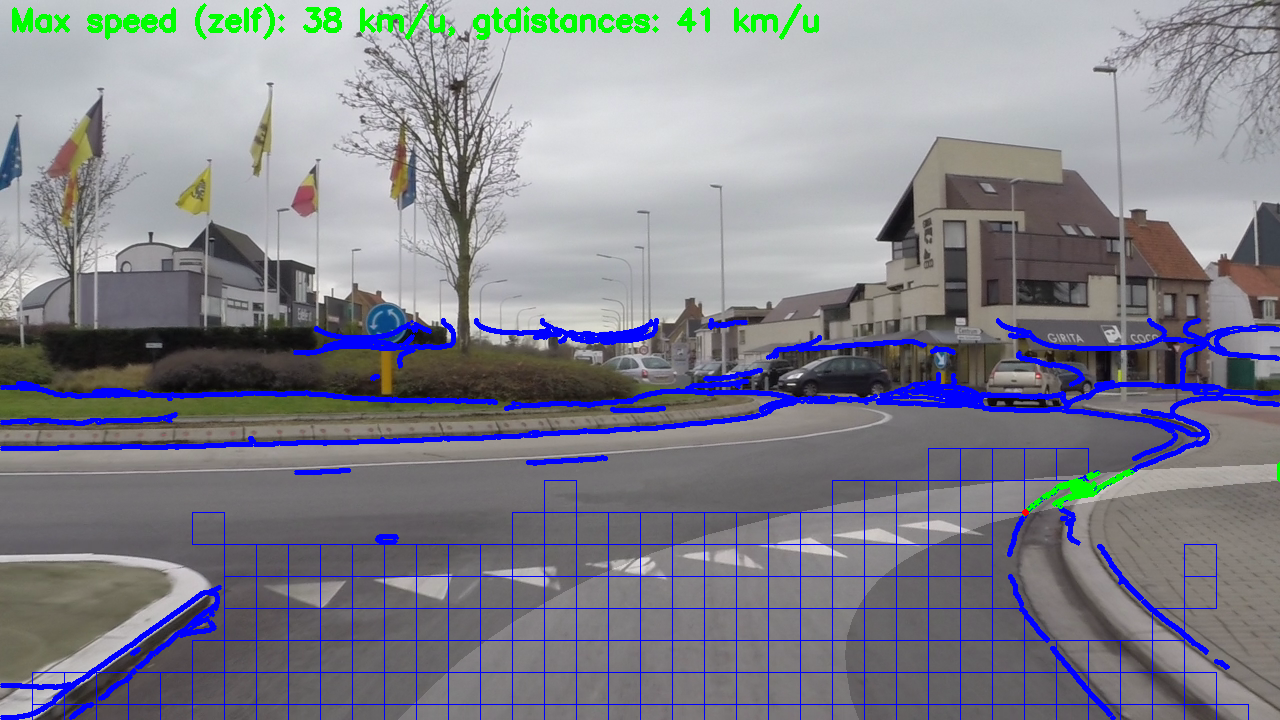
\includegraphics[width=.9\textwidth]{fig/frame00025.png}
  \caption{Visualization of a processed frame showing both classification and edge detection}
  \label{visualization}
\end{figure}

\section{Results}

\subsection{SVM classification}\label{results-svm-classification}
We iterated through several parameter values (as discussed in \ref{parameters-classification}) to find optimal classification for road detection. For each combination of parameters we train and test on different combinations of datasets. For each combination we calculate the F-scores. These scores are used to compare the classification results (higher F-scores indicate better classification). 

todo: geen schatten van edge detection meer

Of the four datasets, different combinations of training sets were selected (each time shown as x-axis on the graphs). The trained classifier was then tested on the remaining datasets.

\subsubsection{Kernels}
As previously mentioned in section \ref{methods-kernels}, there are two SVM kernels we can use for this classification problem. On average, we tend to get a nearly 11\% increase in F-scores using RBF kernel instead of linear kernel. It is safe to say the RBF kernel outperforms the linear kernel for this classification problem in all of our test scenarios. 

\subsubsection{Block size}
In general, block sizes 16x16px and 32x32px tend to show the better results. As an example we present the F-scores for LBP and color with road marks in figure \ref{fig:lbp-col-wi-rm}. Other combinations follow the same trend. For the goal of this application, a smaller block size will be more practical (i.e. better accuracy). This is why prefer the block size of 16x16px. 

\begin{figure}
\centering
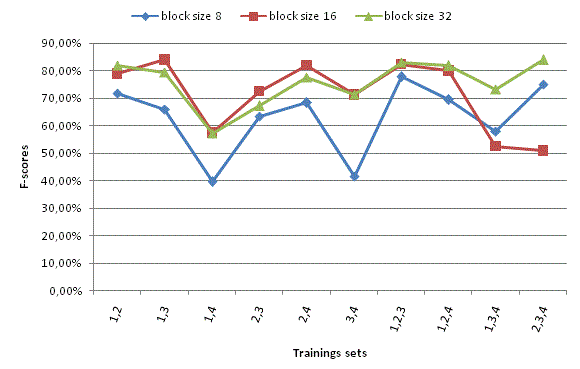
\includegraphics[width=\textwidth]{fig/RBF_LBP_Col_wi_RM.png}
\caption{F-scores for LBP and color with road marks using RBF kernel}
\label{fig:lbp-col-wi-rm}
\end{figure}

\subsubsection{LBP}
The use of LBP is crucial to our implementation in order to get a viable classifier for road detection. If we compare results (block size 16x16px) of feature vectors on LBP only to the combination of LBP and color, we get different results depending on whether or not we include road marks. 

If we do not include road marks in the training data, we get slightly better results when combining LBP and color for the feature vectors (as shown in figure \ref{fig:16_wo_roadmarks}).
If on the other hand we do include these road marks, using only LBP shows equal or better results than the combination of LBP and color (as shown in figure \ref{fig:16_wi_roadmarks}). 

\begin{figure}[h]
\centering
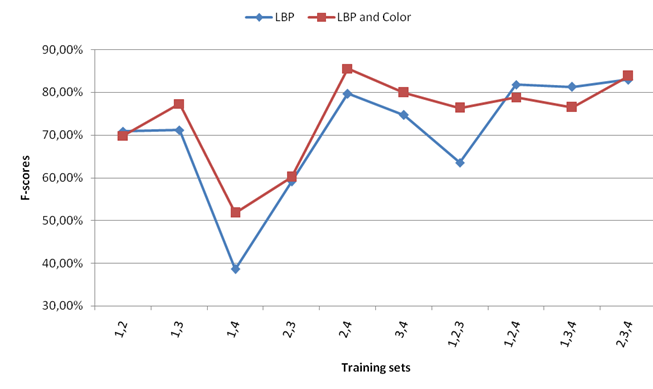
\includegraphics[width=\textwidth]{fig/16_wo_roadmarks.png}
\caption{Comparision of F-scores for 16x16px block size without road marks using RBF kernel }
\label{fig:16_wo_roadmarks}
\end{figure}

A possible explanation for this phenomenon is that when only asphalt is considered to be road, color is a much more consistent factor to weigh in to the classification. However when including road marks as part of the road, color intensity is no longer an added value and even tends to mislead the classifier. 

Overall we can conclude that using only LBP with road marks shows the optimal results for our classification problem. 

\begin{figure}[h]
\centering
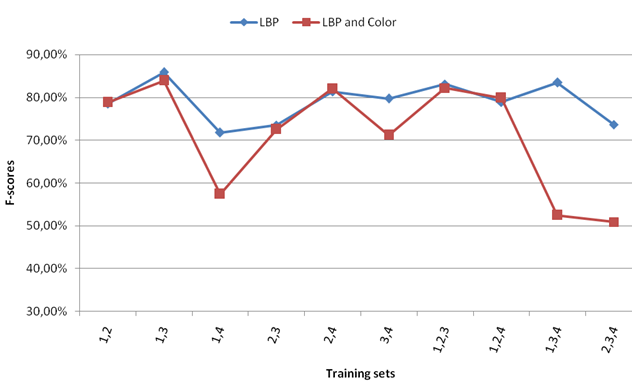
\includegraphics[width=\textwidth]{fig/16_wi_roadmarks.png}
\caption{Comparision of F-scores for 16x16px block size with road marks using RBF kernel }
\label{fig:16_wi_roadmarks}
\end{figure}

Considering the results of the different scenarios, we can conclude that training on dataset four results in poorer classification overall. This is because another type of road is used in this dataset, conflicting with the more common road type present in the other datasets. This distorts the classifier increases misclassifications.

\textbf{TODO} check if list not f***ed up.\\
\noindent In retrospect, the optimal parameters for our classification problem are:
\begin{itemize}
\item RBF kernel
\item Block size 16x16px
\item Using only LBP histogram values for the feature vectors
\item Including road marks as part of the road  
\end{itemize}

\subsection{Driving results}
Driving results get evaluated using a script that calculates the distance a vehicle can drive in one minute, based on the given speed by our system. This script includes a ''ground truth'' for each frame in each dataset. If our speeds exceed this ground truth, the vehicle crashes and is not able to continue driving.

In section \ref{method-combination} two strategies were presented. These use a combination of classification and edge detection. First, the evaluation was run separately on these two methods. The results are shown in figure \ref{distance_result}. The first bar of the histogram shows for every dataset the performance of road classification. Because of a crash in the first dataset there can only be traveled 317m (out of the 1350m). The second bar shows for each dataset the distance traveled only relying on edge detection. There are no crashes in the four datasets so we can say these results are way better. This makes us believe the second combination strategy will be the better one, as it relies.

TODO: maximum met edge detection voor elke dataset? 1350, 

The first way of combining the two methods is very safe and thus results in no crashes over the four datasets. A region is considered to be road only if it's identified as road by the road classification and if there are no edges. Both classification and edge detection should indicate a pixel as road in order to be used for safe driving. The performance of this combination is shown in the third bar of figure \ref{distance_result}. As said, this strategy is very safe, giving up a lot of traveled distance in favor of safety. 

The second strategy for combination also results in zero crashes over the four datasets. This strategy tries to focus on edge detection. A region is considered road if there are no edges. When there are edges, road classification is used to decide whether it's road or not. This strategy gave us the best results, as shown in figure \ref{distance_result} as the fourth bar.
\begin{figure}[ht]
	\centering
	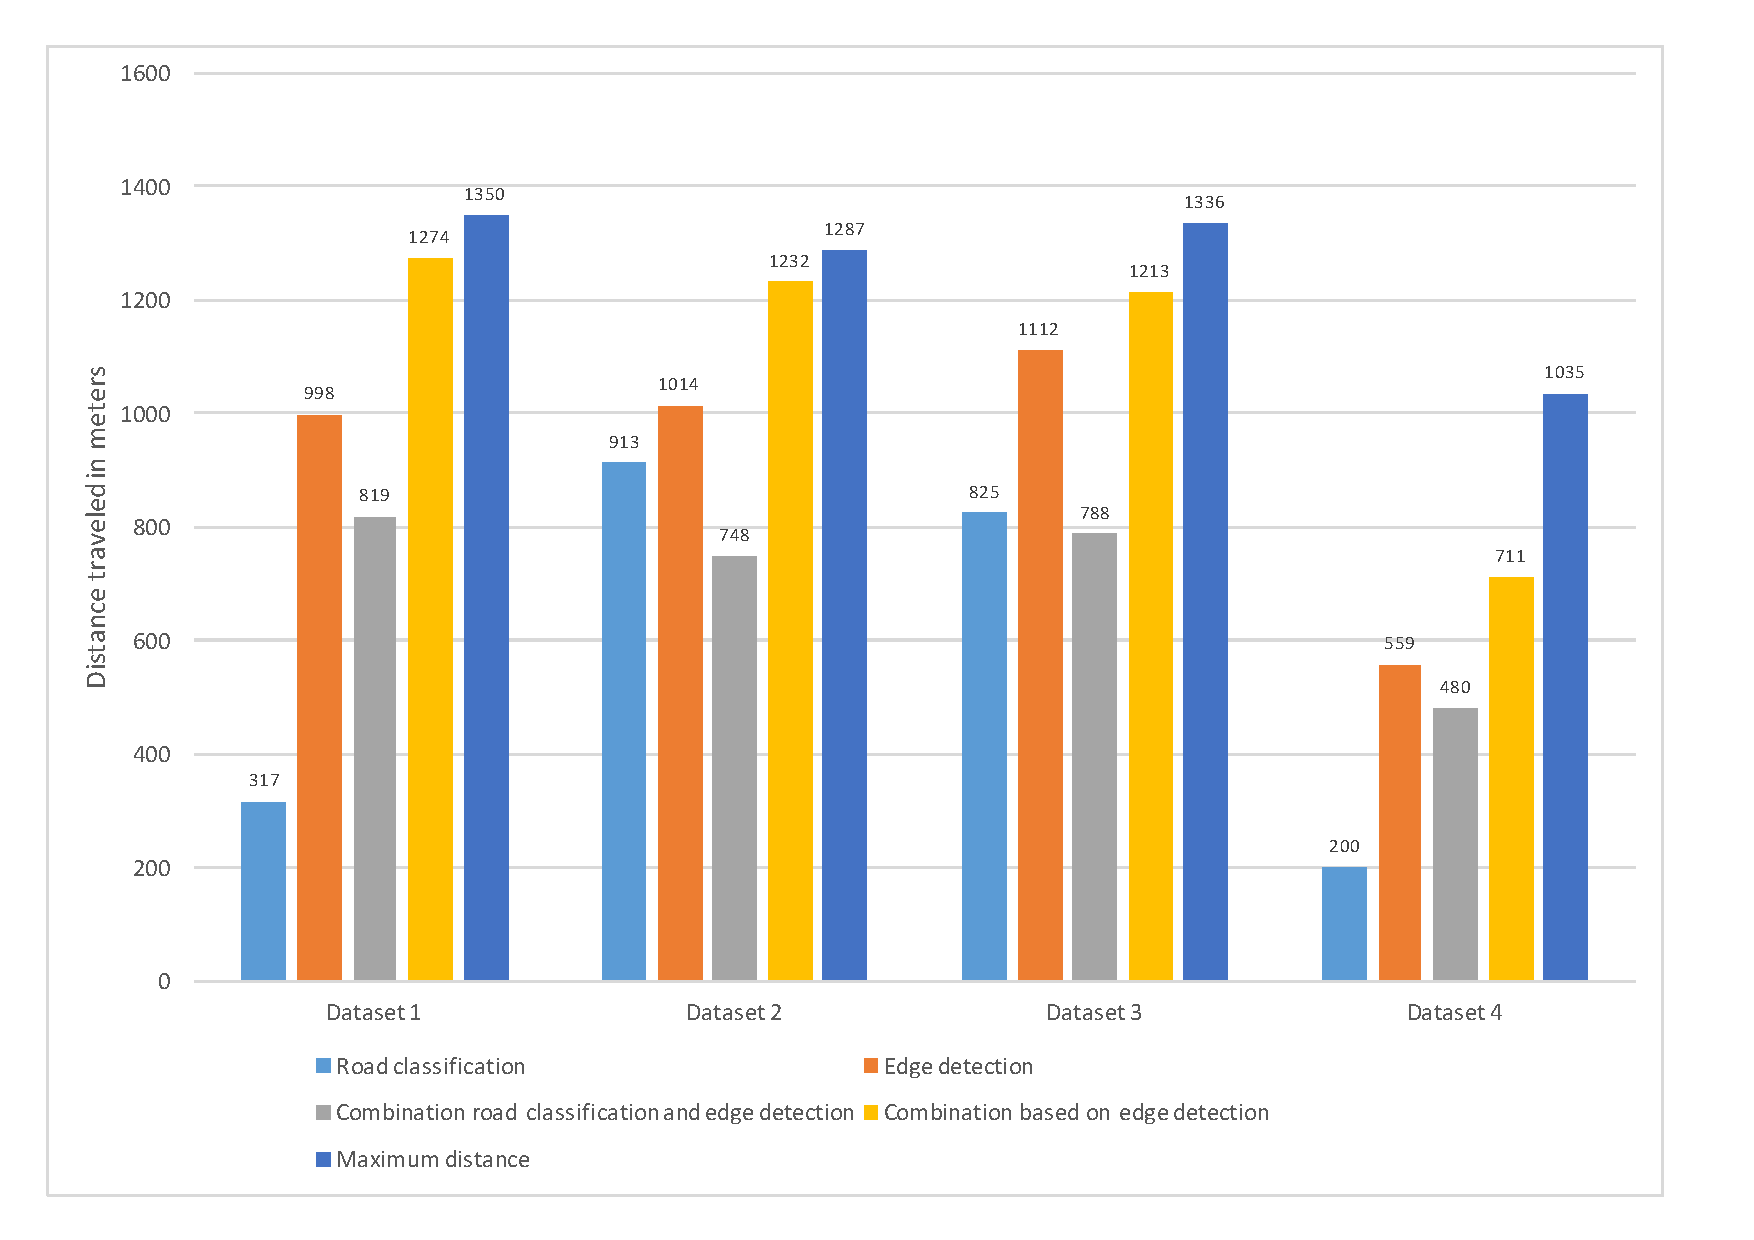
\includegraphics[width=\textwidth]{fig/distance_result}
	\caption{Results of road classification, edge detection and combinations.\label{distance_result}}
\end{figure}



As an extra, this strategy is also able to cope better with zebra crossings than the first strategy. This is shown in figure \ref{zebra}. In the first figure (\ref{zebra-1}) TODO

\begin{figure}[t]
\centering
\begin{subfigure}[t]{.5\textwidth}
  \centering
  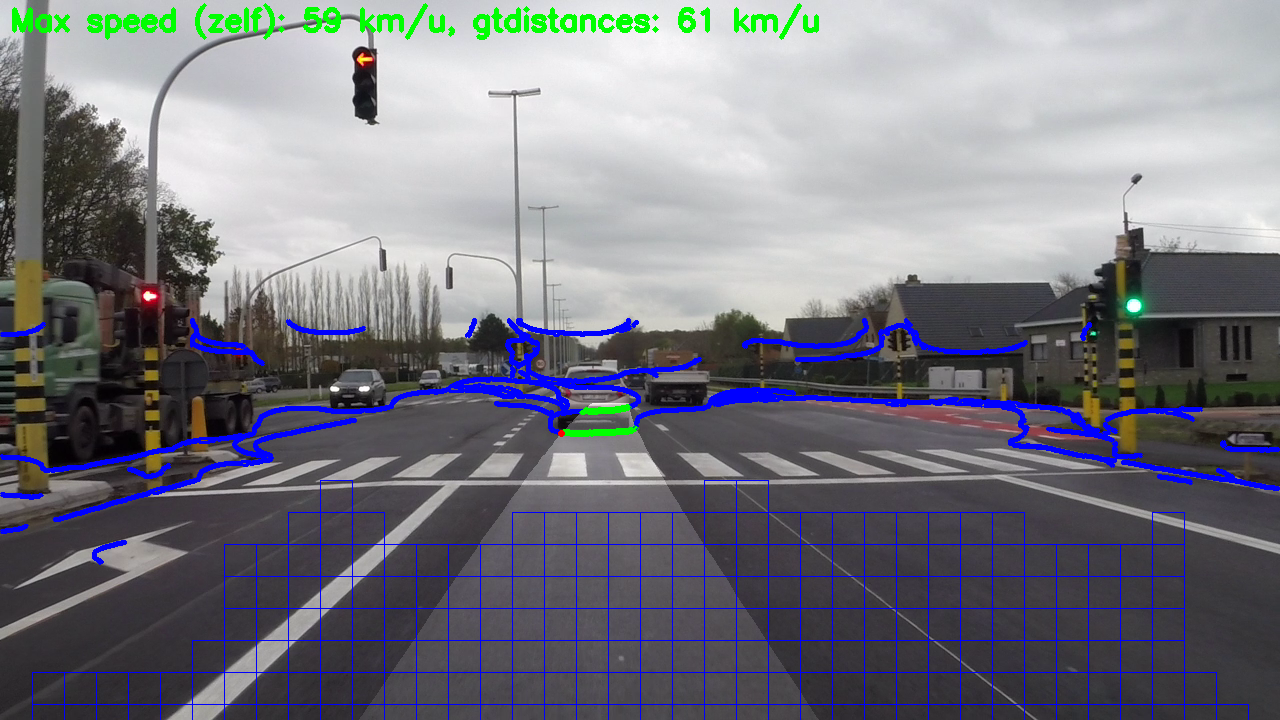
\includegraphics[width=.9\textwidth]{fig/zebra_edge_filtered.png}
  \caption{Zebra crossing filtered out by edge detection.}
  \label{zebra-1}
\end{subfigure}%
\begin{subfigure}[t]{.5\textwidth}
  \centering
  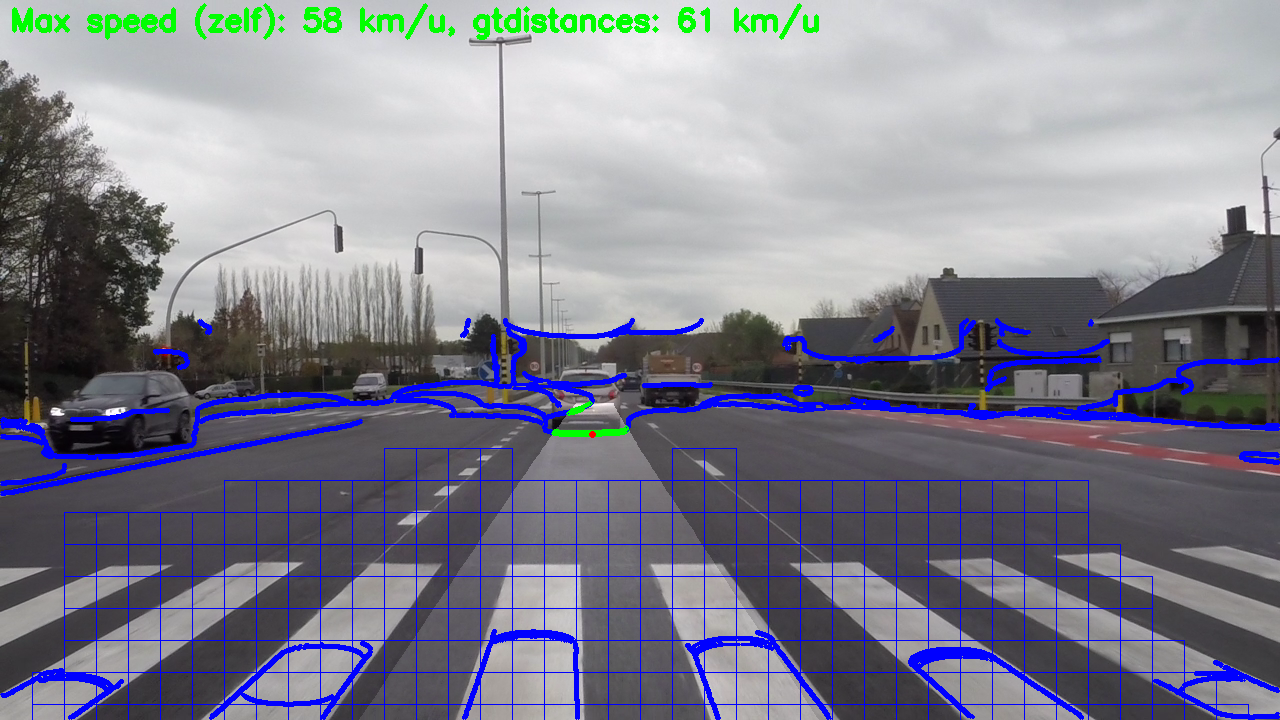
\includegraphics[width=.9\textwidth]{fig/zebra_road_filtered.png}
  \caption{Zebra crossing classified as road.}
  \label{zebra-2}
\end{subfigure}
\caption{Zebra crossing\label{zebra}}
\end{figure}

\section{Conclusion}
\newpage
\bibliography{Computervisie}{}
\bibliographystyle{plain}

\end{document}
